%!TEX root = ./virology.tex

\section{History}

Human rotavirus (RV) was discovered in 1973 by Bishop et al. utilizing direct visualization by electron microscopy. Approximately concurrently, simian, murine, O, and bovine agents were discovered that later would be additionally classified as rotaviral.

\section{Classification}

RVs comprise the genus \textit{Rotavirus} within the family \textit{Reoviridae}. Some features are that:

\begin{enumerate}
	\item the mature viruses are about $100$nm ($1,000$\AA) in diameter with a triple-layered icosahedral protein capsid being comprised of outer and intermediate layers and an inner core;
	\item 60 protein spikes protrude from the outer shell;
	\item calcium is required to maintain the integrity of the outer shell;
	\item particles contain an RNA-dependent RNA polymerase and related enzymes able to produce capped RNA transcripts;
	\item the virus genome contains 11 dsRNA segments;
	\item genetic reassortment can occur between two rotaviruses of the same group; and
	\item the virus particles, uniquely, are formed by migration into the ER where enveloped particles are formed.
\end{enumerate}

RVs are classified into serogroups of multiple serotypes each. An RV group includes viruses that share cross-reacting antigens. There are 7 distinct groups that rotaviruses compose. Group A, B, and C RVs are found in both humans and animals; group D, E, F, and G RVs have only been observed in animals to date.

Group A RVs have been predominantly identified as causing diarrheal disease in infants and mammalian and avian young. Group B RVs are associated with severe diarrheal epidemics. Group C RVs have been occasionally reported in family outbreaks.

\clearpage
\begin{landscape}
{\bfseries \large Table 1.} \\
\begin{tabular}{rr|lllp{4.5in}}
\hline
\parbox[t]{0.5in}{Genome\\Segment} & \parbox[t]{0.55in}{Protein Product} & Location & N/virion & \parbox[t]{0.7in}{Ts mutant group} & Function \\
\hline
1 & VP1 & Core & 12 & C & RNA-dependent RNA polymerase, ss-RNA binding, complex with VP3 \\
2 & VP2 & Core & 120 & F & RNA binding, required for replicase activity of VP1 \\
3 & VP3 & Core & 12 & B & Guanylytransferase, methytransferase, ss-RNA binding, complex with VP1 \\
4 & VP4 & Outer capsid & 120 & A & Hemagglutinin, cell attachment, neutralization antigen, protease enhanced infectivity, virulence, putative fusion region \\
5 & NSP1 & Nonstructural & & NA & Basic, zinc finger, RNA binding, virulence in mice; interacts with and degrades IRF-3; nonessential for some strains \\
6 & VP6 & Inner capsid & 780 & G & Hydrophobic, trimer, subgroup antigen, protection; required for transcription \\
7 & NSP3 & Nonstructural & & NA & Acidic dimer, binds $3^{\prime}$ end of viral mRNAs, competes with cellular PABP for interaction with elF-4G1, inhibits host translation \\
8 & NSP2 & Nonstructural & & E & Basic, RNA binding, oligomer, NTPase, helicase, forms viroplasms with NSP5 \\
9 & VP7 & Outer capsid & 780 & NA & RER integral membrance glycoprotein, calcium-dependent trimer, neutralization antigen \\
10 & NSP4 & Nonstructural & & NA & RER transmembrance glycoprotein, intracellular receptor for DLPs, wole in morphogenesis, interacts with viroplasms, modulates intracellular calcium and RNA replication, enterotoxin, secreted cleavage product, protection by antibody, virulence \\
11 & NSP5 & Nonstructural & & NA & Basic phosphoprotein, RNA binding, protein kinase, forms viroplasms with NSP2, interacts with VP2 and NSP6 \\
& NSP6  & Nonstructural & & NA & Interacts with NSP5, present in viroplasms and most virus strains \\
\hline
\end{tabular} \\
{\itshape Note.} Table of rotavirus proteins and their relevant data. Adapted from Fields Biology, 5e.
\end{landscape}
\clearpage

\section{Virion Structure}

Three-dimensional reconstructions using cryo-electron microscopy have revealed that RV particles possess icosahedral symmetry with a $T=13l$ icosahedral surface lattice for the two outer layers. There exist also $132$ large channels $\sim 140\AA$ deep that span both shells and link the outer surface with the inner core (Figure \ref{fig01}.

\begin{figure}[htp]
\begin{center}
% Define decoration
\pgfdeclaredecoration{outerCapsid}{initial}
{
  \state{initial}[width=\pgfdecoratedpathlength/floor(\pgfdecoratedpathlength/7pt)]
  {
    % Draw the two legs
    \pgfpathmoveto{\pgfpoint{-1pt}{0pt}}
    \pgfpathlineto{\pgfpoint{-1pt}{-10pt}}
    \pgfpathmoveto{\pgfpoint{1pt}{0pt}}
    \pgfpathlineto{\pgfpoint{1pt}{-10pt}}
    % Draw the head group
    \pgfpathmoveto{\pgfpoint{1pt}{0pt}}
    \pgfpathcircle{\pgfpoint{0pt}{2pt}}{2.5pt}
  }
  \state{final}
  {
    \pgfpathmoveto{\pgfpointdecoratedpathlast}
  }
}

\pgfdeclaredecoration{intermediate}{initial}
{
  \state{initial}[width=\pgfdecoratedpathlength/floor(\pgfdecoratedpathlength/7pt)]
  {
	\draw [fill = red!50] (2pt,3pt) -- (-2pt,3pt) -- (-1pt, 0pt) -- (-2pt, -3pt) -- (2pt, -3pt) -- (1pt, 0pt) -- cycle;
  }
  \state{final}
  {
    \pgfpathmoveto{\pgfpointdecoratedpathlast}
  }
}

\pgfdeclaredecoration{inner}{initial}
{
  \state{initial}[width=\pgfdecoratedpathlength/floor(\pgfdecoratedpathlength/8pt)]
  {
\draw [fill = blue!50] (2.5pt,0pt) -- (0pt,2.5pt) -- (-2.5pt,0pt) -- (0pt,-2.5pt) -- cycle;
  }
  \state{final}
  {
    \pgfpathmoveto{\pgfpointdecoratedpathlast}
  }
\pgfusepath{fill,stroke}
}

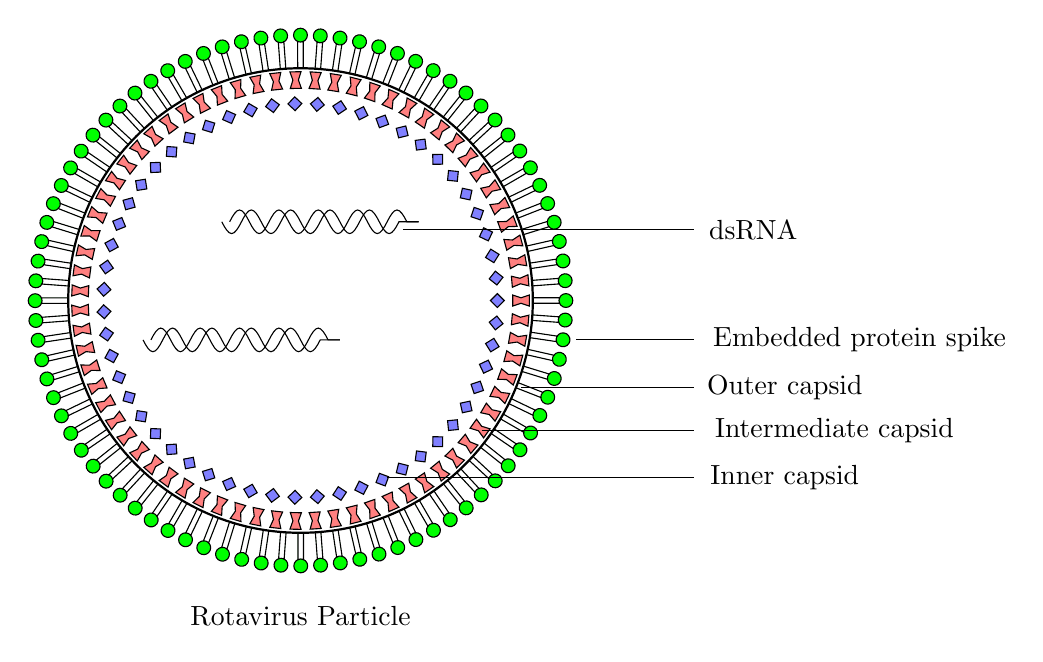
\begin{tikzpicture}
% Rotavirus
\draw[decorate, decoration={inner}] (5, 0.5) circle (2.5cm);
\draw[decorate, decoration={intermediate}] (5, 0.5) circle (2.8cm);
\draw[decorate, thick] (5, 0.5) circle (2.95cm);
\draw[decorate, fill=green, decoration={outerCapsid, mirror}] (5, 0.5) circle (3.3cm);
\draw (5, -3.5) node {Rotavirus Particle};
\draw[decorate, decoration={coil, aspect=0, segment length=0.5cm, amplitude=.15cm}] (3.1,0) -- (5.5,0);
\draw[decorate, decoration={coil, aspect=0, segment length=0.5cm, amplitude=-.15cm}] (3,0) -- (5.5,0);
\draw[decorate, decoration={coil, aspect=0, segment length=0.5cm, amplitude=.15cm}] (4.1,1.5) -- (6.5,1.5);
\draw[decorate, decoration={coil, aspect=0, segment length=0.5cm, amplitude=-.15cm}] (4,1.5) -- (6.5,1.5);
\draw (6.3,1.4) -- (10,1.4);
\node at (10.75,1.4) {dsRNA};
\draw (8.5,0) -- (10,0);
\node at (12.1,0) {Embedded protein spike};
\draw (7.8,-0.6) -- (10,-0.6);
\node at (11.15,-0.6) {Outer capsid};
\draw (7.3,-1.15) -- (10,-1.15);
\node at (11.78,-1.15) {Intermediate capsid};
\draw (6.1,-1.75) -- (10,-1.75);
\node at (11.15,-1.75) {Inner capsid};
\end{tikzpicture}
\end{center}
\caption{Schematic illustration of a rotavirus particle, laterally bisected.}
\label{fig01}
\end{figure}

Three types of channels have been identified based on position and size. Specifically, there are $12$ type I channels running down the icosahedral fivefold axes; 60 type II channels around the fivefold axes; and 60 type III channels around the threefold icosahedral axes.

Further, 60 spikes extend from the surface of he outer shell. These protein spikes lit on the edges of the type II channels and are composed of VP4. The spikes have a distinct structure with two distal globular head domains, a central body, and an internal globular domain tucked inside the VP7 layer in the type II channels.  

\section{Genome Structure}

The viral genome of 11 dsRNA segments is contained within the core capsid. The virus particles have been shown to contain their own RNA-dependent RNA polymerase to transcribe the individual RNA segments into active mRNA. (I.e., deproteinized RV dsRNA are non-infectious.)

Each positive-sense RNA segment starts with a $5^{\prime}$-guanidine followed by a set of conserved sequences that are part of the $5^{\prime}$-noncoding sequences. An open reading frame (ORF) coding for the protein product and ending with the stop codon follows, and then another set of noncoding sequences is found containing a subset of conserved terminal $3^{\prime}$-terminal cytidines.

\begin{figure}[htp]
	\begin{center}
		\begin{tikzpicture}
		% Left noncoding region
		\draw [pattern = north west lines] (0in,0in) -- (0in,0.25in) -- (0.5in,0.25in) -- (0.5in,0in) -- cycle;
		% ORF
		\draw [fill = white] (0.5in,0in) -- (3.5in,0in) -- (3.5in,0.25in) -- (0.5in,0.25in) -- cycle;
		\node [draw = none] at (2in,0.4in) {ORF};
		% Right noncoding region
		\draw [pattern = north west lines] (3.5in,0in) -- (4in,0in) -- (4in,0.25in) -- (3.5in,0.25in) -- cycle;
		% Left noncoding upper label
		\draw (0in,0in) -- (0in,0.4in);
		\draw (0.5in,-0.1in) -- (0.5in,0.4in);
		\node [draw = none, align = center] at (0.25in,0.6in) {Noncoding\\ (9-48)};
		% AUG label
		\node [draw = none] at (0.5in, -0.2in) {AUG};
		% 2nd AUG label
		\draw (1.2in, 0in) -- (1.2in, -0.3in);
		\node [draw = none, align = center] at (1.2in, -0.5in) {(2nd in-phase or\\ out-of-phase AUG)};
		% Right noncoding upper label
		\draw (3.5in,0in) -- (3.5in, 0.4in) -- (3.7in, 0.5in);
		\node [draw = none, align = center] at (4in, 0.6in) {Noncoding\\ (17-182)};
		% Cis-regulatory element labels
		\draw (4in,0in) -- (4in,-0.1in) -- (4.5in, -0.2in);
		\draw (3.9in,0in) -- (3.9in, -0.1in) -- (3.3in,-0.2in);
		\node [draw = none, align = center] at (3.9in, -0.3in) {\scriptsize {UUAAGUUAGAACUGUAUGAUGUGACC}};
		\node [draw = none, align = left] at (3.3in, -0.6in) {$3^{\prime}$-enhancing \\ sequence};
		\node [draw = none, align = center] at (3.8in,-0.5in) {\large {$|$}};
		\node [draw = none, align = right] at (4.5in,-0.5in) { Minimal promoter};
		\draw[<->, line width = 2pt] (3in, -0.875in) -- (4.8in, -0.875in);
		\node [draw = none, align = center] at (3.9in, -1in) {{\itshape cis}-regulatory elements};
		\end{tikzpicture}
	\end{center}
\caption{Major features of rotavirus gene structure. Schematic shows the overall structure of RV genes derived from published sequences of genes 1 through 11. All 11 RV genes lack a polyadenylation signal, are A+U righ, and contain conserved consensus sequences at their $5^{\prime}$ and $3^{\prime}$ ends.}
\label{fig02}
\end{figure}

One of the most intriguing aspects of RV replication relates to the mechanism(s) of how it coordinately replicates and packages the 11 viral mRNAs. These 11 mRNAs must share common cis-acting signals because they are all replicated by the same polymerase, and the UGUG sequence of the consensus sequence is reorganized in a base-specific manner by the polymerase. Additionally, each mRNA must contain a signal that is unique to it alone because the 11 mRNA must be distinguished from one another during packaging. Generally, the conserved terminal sequences in genome segments contain cis-acting signals that are important for the transcription, RNA translation, RNA transport, replication, assembly, or encapsidation of the viral genome segments. Some of the cis-acting signals for RV RNA replication and translation have been identified (Figure \ref{fig02}), but assembly or encapsidation signals remain unknown. The highly conserved noncoding regions of the RNA may contain the gene-specific packaging signals.

\section{Coding Assignments}

\section{Stages of Replication}

\section{Pathogenesis and Pathology}

\section{Epidemiology}

\section{Immunity}

\section{Clinical Features and Diagnosis}

\section{Prevention and Control}